% !TEX encoding = UTF-8 Unicode
\documentclass[a4paper]{article}

\usepackage[utf8]{inputenc}
\usepackage{erk}
\usepackage{times}
\usepackage{graphicx}
\usepackage[top=22.5mm, bottom=22.5mm, left=22.5mm, right=22.5mm]{geometry}
\usepackage{amsmath}
\usepackage[slovene,english]{babel}

% local definitions
\def\footnotemark{}%  to avoid footnote on cover page

\begin{document}
%make title
\title{Mean shift sledilnik s Kalmanovim filtrom}

\author{Ivan Antešič} % use ^1, ^2 for author(s) from different institutions

\affiliation{Fakulteta za računalništvo in informatiko, \\
Univerza v Ljubljani, \\
Večna pot 113, Ljubljana }

\email{E-pošta: ivan.v.antesic@gmail.com}

\maketitle

%\thispagestyle{empty}

\begin{abstract}{Povzetek}
Izpeljali smo Kalmanov filter in pokazali njegovo delovanje na praktičnem primeru sledenja tarči z Mean shift sledilnikom. %Testirali smo različne modele gibanja na večih sekvencah slik in komentirali njihov vpliv.  
Da bi izboljšali delovanje in preprečili odpovedi pri zakritju tarče smo sledilniku dodali Kalmanov filter. S testiranjem različnih modelov gibanja in parametrov smo ugotovili, da lahko z dinamičnim modelom izboljšamo delovanje pri specifičnih primerih. 
%Na koncu so povzete še glavne ugotovitve.
\end{abstract}

\selectlanguage{slovene}

\section{Uvod}
Kalmanov filter je algoritem poimenovan po Rudolfu E. Kálmánu, ki za določitev stanja tarče uporablja Bayesove principe verjentosti. S kombiniranjem meritve in predikcije zgladi morebitno šumne meritve ter tako bolj natančno določi naslednje stanje. Pogosto se uporablja se pri navigaciji, kontroli vozil, vodenju procesov, procesiranju signalov in ekonometriki. V okviru seminarske naloge smo Kalmanov filter uporabili na problemu računalniškega vida in v Mean shift sledilnik vpeljali Kalmanov filter.

Mean shift sledilnik, v večini primerov deluje razmeroma dobro. Barvni vizuelni model histograma je robusten in neobčutljiv na različne transformacije tarče. Še vedno pa ima sledilnik težave z delno ali popolno zakritostjo tarče (angl. occlusion) ter zamenjavo tarče za podobno obarvan predmet v bližini. Te težave, bi lahko ublažili z uvedbo modela gibanja. Zato smo se odločili, da nadgradimo sledilnik s Kalmanovim filtrom. 

Kalmanov filter omogoča predvidenje dobre začetne točke Mean shift algoritma, kar se odraža v boljši lokalizaciji - lažje dosežemo globalni maksimum. Ko so meritve Mean shifta nezaneslijive (zakrita tarča ali napačna zaznava), zaradi upoštevanja dinamičnega modela predvidimo kje se v resnici nahaja tarča in tako ohranimo sledenje. Sledenje je manj šumno, saj se povprečijo meritve Mean shift sledilnika in napovedi dinamičnega modela. 

\section{Kalmanov filter}
Delovanje in teorija Kalmanovega filtra je opisana v knjigi \cite{prince} s katero smo si pomagali pri razumevanju in implementiranju algoritma. 

%\subsection{Izpeljava}
Definirajnmo spremenljivki stanje $w_t$ za dinamični model in meritev $x_t$ za model meritev.
\subsection{Dinamični model} 
Dinamični model definira povezavo stanja $w_t$ ob času $t$ s stanjem ob času $t_{-1}$ kot: $$w_t = \Psi*w_{t-1} + \epsilon_p$$ 
Stanje smo predstavili z vektorjem x in y komponent:
\begin{itemize}
	\item položaja
	\item hitrosti (časovnim odvodom položaja) 
	\item pospeška (časovnim odvodom hitrosti) 
	\item pri modelu NCA še dodatno s sunkom (časovnim odvodom pospeška)
\end{itemize}

$$
w_t=
\begin{bmatrix}
	x\\y\\\dot{x}\\\dot{y}\\\ddot{x}\\\ddot{y}
\end{bmatrix}
,\dot{w_t}=
\begin{bmatrix}
	\dot{x}\\\dot{y}\\\ddot{x}\\\ddot{y}\\\dddot{x}\\\dddot{y}
\end{bmatrix}
$$

$\Psi$ je matrika, ki določi katere komponente stanja upoštevamo pri predikciji in je odvisna od modela gibanja, ki ga uporabljamo. $\epsilon_p$ je naključna spremenljivka, ki predstavlja šum določen z matriko kovariance šuma dinamičnega modela $\Sigma_p$.

Da lahko določimo $\Psi$ je torej potrebno najprej definirati model gibanja, ki opisuje gibanje po formuli $\dot{w}=F*w+L* \epsilon$. Za vsak model določimo matriki $F$ (katere komponente upoštevamo) in $L$ (katere komponente so šum).

\subsubsection{RW}
Pri modelu naključne hoje (angl. random walk) je hitrost definirana le s šumom, pospeška in sunka ne upoštevamo. Model je primeren za opis hitrih nenadnih in nepričakovanih sprememb.
$$
\dot{w_t}=
\begin{bmatrix}
	\dot{x}\\\dot{y}\\\ddot{x}\\\ddot{y},
\end{bmatrix}
,F = \begin{bmatrix}
	0&0&0&0\\0&0&0&0\\0&0&0&0\\0&0&0&0
\end{bmatrix}
,L = \begin{bmatrix}
	1&0\\0&1\\0&0\\0&0
\end{bmatrix}
$$

\subsubsection{NCV}
Model skoraj konstantne hitrosti (angl. near constant velocity) opisuje gibanje, ki ima konstanto hitrost in pospešek definiran s šumom. Primeren za objekte, ki se premikajo brez pospeška (npr. avto, ki vozi z isto hitrostjo).
$$
\dot{w_t}=
\begin{bmatrix}
	\dot{x}\\\dot{y}\\\ddot{x}\\\ddot{y},
\end{bmatrix}
,F = \begin{bmatrix}
	0&0&1&0\\0&0&0&1\\0&0&0&0\\0&0&0&0
\end{bmatrix}
,L = \begin{bmatrix}
	0&0\\0&0\\1&0\\0&1
\end{bmatrix}
$$

\subsubsection{NCA}
Model skoraj konstantnega pospeška (angl. near constant acceleration) je predstavljen s konstantno hitrostjo in pospeškom, nenadni sunki pa so definirani s šumom. Primerno za objekte, ki postopoma pospešujejo ali zavirajo svoje gibanje (npr. vzlet letala). 
$$
\dot{w_t}=
\begin{bmatrix}
\dot{x}\\\dot{y}\\\ddot{x}\\\ddot{y}\\\dddot{x}\\\dddot{y},
\end{bmatrix}
,F = \begin{bmatrix}
0&0&1&0&0&0\\0&0&0&1&0&0\\0&0&0&0&1&0\\0&0&0&0&0&1
\end{bmatrix}
,L = \begin{bmatrix}
0&0\\0&0\\0&0\\0&0\\1&0\\0&1
\end{bmatrix}
$$
Sedaj lahko določimo matriko $\Psi$ po enačbi: $\Psi = e^{L*\Delta t}$. Enačbo smo izračunali, kar z uporabo Matlab paketa \textit{Symbolic toolbox}. S paketom izračunamo tudi kovariančno matriko $\Sigma_p = \int_0^{\Delta t} (\Psi(\xi)L)k_q(\Psi(\xi)L)^{T}d\xi$. Za npr. NCV model in $\Delta t=1$ bi bili matriki enaki:
$$
\Psi=
\begin{bmatrix}
	1&0&1&0\\0&1&0&1\\0&0&1&0\\0&0&0&1
\end{bmatrix}
,\Sigma_p = k_q*\begin{bmatrix}
	1/3&0&1/2&0\\0&1/3&0&1/2\\1/2&0&1&0\\0&1/2&0&1
\end{bmatrix}
$$ 
$k_q$ je parameter s katerim določimo velikost $\Sigma_p$.
 
\subsection{Model meritev} 
$x_t$ je meritev, ki jo vrne Mean shift sledilnik, definirana kot $$x_t = \Phi*w_{t} + \epsilon_m$$ V našem primeru meritev vsebuje le položaj v x in y koordinatah.
$$
x_t=
\begin{bmatrix}
x\\y\\
\end{bmatrix}
$$
Matrika $\Phi$ iz stanja $w_t$ izloči položaj tarče, $\epsilon$ pa predstavlja šum določen z matriko kovariance šuma meritvenega modela $\Sigma_m$. Za npr. NCV model, bi bili matriki enaki:
$$
\Phi=\begin{bmatrix}
	1&0&0&0\\0&1&0&0
\end{bmatrix}
,\Sigma_m = k_r*\begin{bmatrix}
	1&0\\0&1
\end{bmatrix}
$$
$k_r$ je parameter s katerim določimo velikost $\Sigma_m$.

\subsection{Inferenca} 
Kalmanov filter po naslednji formuli definira verjetnost, da smo prišli v stanje $w_t$ glede na meritve $x_{1:t}$:
\begin{align*}
&p(w_t\mid x_{1:t}) \propto\\ 
&p(x_t\mid w_t)\int p(w_t\mid w_{t-1})p(w_{t-1}\mid x_{1:t-1})dw_{t-1}
\end{align*}
Iz prejšnega stanja (previous posterior) $p(w_{t-1}\mid x_{1:t-1})$ z modelom gibanja $p(w_t\mid w_{t-1})$ naredi predikcijo stanja (prior) $p(w_{t}\mid x_{1:t-1})$. To nato združimo z meritvijo $p(x_t\mid w_t)$ v novo stanje (posterior). V naslednji iteraciji postane posterior prejšne stanje. Postopek je vizuelno predstavljen na sliki \ref{kalman}.

Kalmanov filter predpostavi, da so vse verjetnosti formule predstavljene s funkcijo Gaussove porazdelitve in s tem upošteva negotovost stanj tarče. Tako je npr. meritev predstavljena kot: $p(x_t\mid w_t) = G(\mu_m = \psi*w_t, \Sigma_m)$.

\begin{figure}[h]
	\begin{center}
		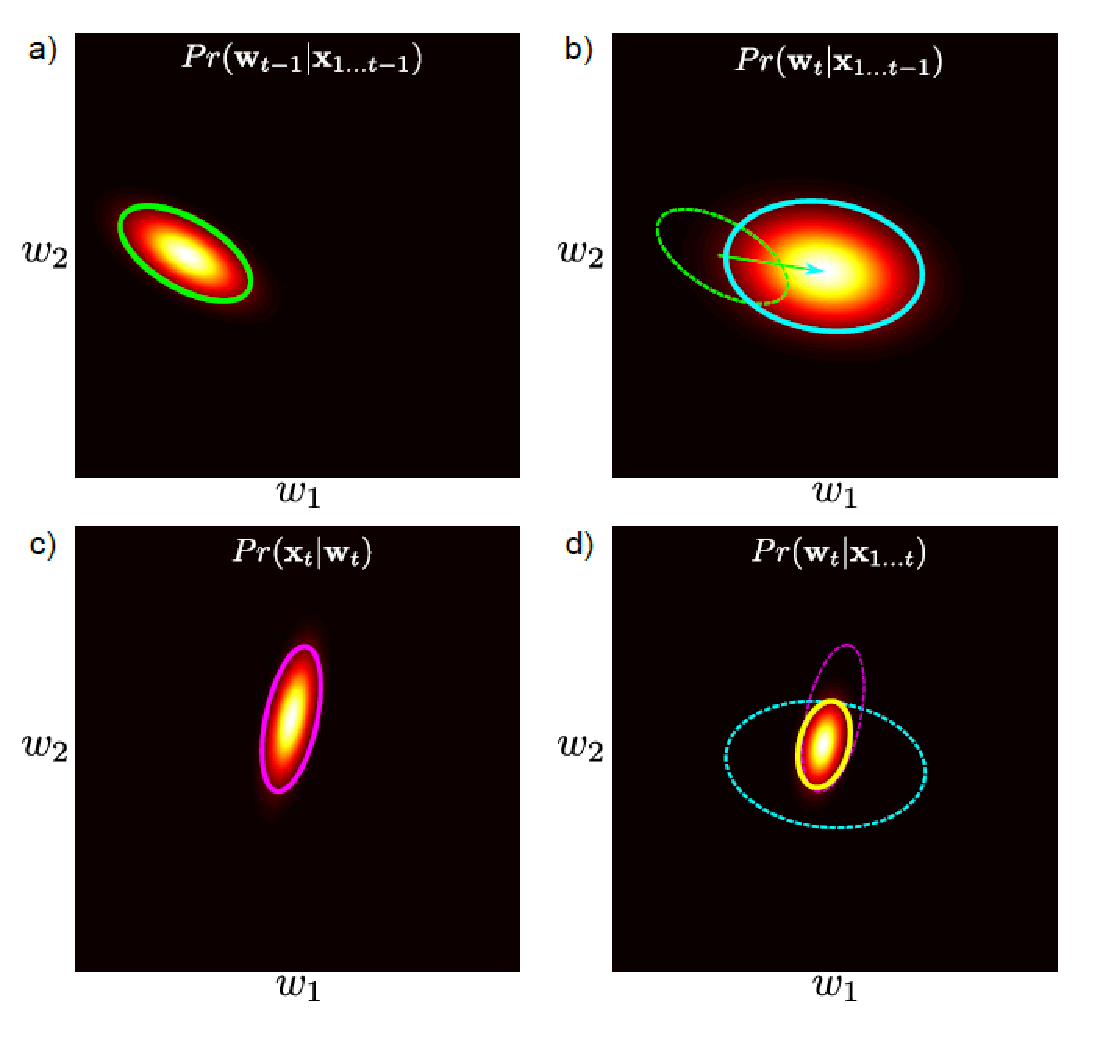
\includegraphics [width=0.5\textwidth] {kalman.pdf}
	\end{center}
	\caption{Slika prikazuje delovanje Kalmanovega filtra. V a.) vidimo prejšno stanje, iz katerega predividimo prior v b.). c.) je meritev, ki skupaj z b.) določa novo stanje v d.).}
	\label{kalman}
\end{figure}

Nov posterior izračunamo z Bayesovim pravilom verjetnosti:
\begin{align*}
&p(w_t\mid x_{1:t}) = \frac{p(x_t\mid w_t)p(w_{t}\mid x_{1:t-1})}{p(x_{1:t})}\\
&=\frac{G(\mu_m + \Phi w_t, \Sigma_m)G(\mu_+, \Sigma_+)}{p(x_{1:t})}\\
&=G[(\Phi^T \Sigma_m^{-1} \Phi+\Sigma_+^{-1})^{-1}\\
&((\Phi^T \Sigma_m^{-1}(x_t-\mu_m)+\Sigma_+^{-1}\mu_+)^{-1}),\\
&(\Phi^T \Sigma_m^{-1} \Phi+\Sigma_+^{-1})^{-1}]\\
&=G(\mu_t, \Sigma_t)
\end{align*}
$\Sigma_+$ in $\mu_+$ sta varianca in povprečje stanja predikcije (prior). Ker je računanje novega stanja v tej obliki numerično zahtevno, preoblikujemo enačbo in definiramo Kalmanovo pridobitev.

\subsection{Kalmanova pridobitev}
S Kalmanovo pridobitvijo 
$$K = \Sigma_+ \Phi^T(\Sigma_m + \Phi \Sigma_+\Phi^T)^{-1}$$ 
lahko lažje določimo povprečje $\mu_t$ in varianco $\Sigma_t$ za novo stanje (posterior) $p(w_t\mid x_{1:t}) = G(\mu_t, \Sigma_t)$. 

\begin{align*}
\mu_+ &= \mu_p+\Psi\mu_{t-1}\\
\Sigma_+ &= \Sigma_p + \Psi\Sigma_{t-1}\Psi^T\\
\mu_t &= \mu_+ + K(x_t - \mu_m - \Phi\mu_+)\\
\Sigma_t &= (I - K\Phi)\Sigma_+
\end{align*}

Če je Kalmanova pridobitev velika pomeni, da so meritve bolj zanesljive, kot predikcija in jih bolj upoštevamo. To lahko vidimo tudi iz enačbe za varianco: ko so meritve bolj zanesljive se varianca zmanjša. Kalmanov filter si lahko predstavljamo kot zelo dobro uteženo povprečje meritve in napovedi modela.

Na delovanje Kalmanovega filtra ponavadi vplivamo z nastavitvijo parametra $k_q$ s katerim določamo velikost kovariančne matrike za dinamični model $\Sigma_p$ in s parametrom $k_r$ s katerim določamo velikost kovariančne matrike za meritveni model $\Sigma_m$. Večji $k_q$ bo povečal šum dinamičnega modela in predikcija se bo upoštevala manj. Enako velja za $k_r$ in šum meritev. 

\subsection{Možne izboljšave}
Kalmanov filter deluje dobro dokler model gibanja linearen in imamo le eno hipotezo (Gaussovo funkcijo z enim vrhom), kje se nahaja naše novo stanje. Ker se v praksi velikokrat želimo opisati nelinearna gibanja, na primer. v avtomatiki sisteme, ki poleg položaja in hitrosti upoštevajo še maso, zračni upor, kotno hitrost, ipd., potrebujemo rešiti te probleme z razširitvijo običajnega algoritma.

V našem primeru sledenja tarči skozi sekvenco slik nimamo potrebe po opisu nelinearnega gibanja. Posamezni premiki med zaporednimi slikami so zelo majhni, sistem sledilnika ni kompleksen poleg tega pa ne moremo določiti nelinearni model gibanja, ki bi dobro opisal vse sekvence (saj so si zelo različne). Kljub temu omenimo glavne ideje posameznih izboljšav.

\subsubsection{Razširjeni Kalmanov filter}
Pri razširjenemu Kalmanovem filtru (angl. Extended Kalman filter) lahko opišemo poljubni nelinearni funkciji $f$ in $g$, ki določata stanje in meritev v času $t$:
$$
w_t = f(w_{t-1}, \epsilon_p), x_t = g(w_t, \epsilon_m)
$$
To je možno, ker funkcijo linearno aproksimiramo s Taylorjevim razvojem okoli njenega vrha v $\mu_t$. Dodatno lahko funkcijo zgladimo s ponavljanjem postopka na novih podatkih. Ta pristop imenujemo iterativno razširjeni Kalmanov filter.  

\subsubsection{Neodišavljeni Kalmanov filter}
Z neodišavljenim Kalmanovim filtrom (angl. unscented Kalman filter) lahko opišemo bolj nelinearna gibanja kot z raširjeno obliko. Vendar je potrebno, da je šum gibanja porazdeljen normalno (Gauss). 
$$
w_t = f(w_{t-1}) + \epsilon_p, x_t = g(w_t) + \epsilon_m
$$
Poleg tega postopek ne vsebuje računanja odvodov. Porazdelitve predstavimo z množico sigma točk (Diracovih delta funkcij), ki jih preslikamo z nelinearno funkcijo. Na preslikani množici nato določimo povprečje in kovarianco za normalno porazdelitev. 

\subsubsection{Filter z delci}
Kalmanov filter predpostavi da je verjetnostna funkcija Gaussove oblike. Velikokrat to ne drži, lahko dobimo težjo funkcijo z večimi vrhi. V teh primerih posterior opišemo kot model večih Gaussov (mixture model). Ker ne vemo vnaprej koliko Gaussovih funkcij potrebujemo, iz verjetnostne funkcije vzorčimo veliko Diracovih funkcij. Vzorec vsebuje svojo hipotezo za stanje in utež. Intergriranje nadomestimo z Monte Carlo integracijo ter z računanjem uteži vzorcev dosežemo enako (ampak lažje) vzorčenje težkih funkcij. 

\section{Mean shift sledilnik}
Za lažje razumevanje primera, na kratko opišimo tudi sledilnik, ki smo ga nadgradili s Kalmanovim filtrom. Pri implementaciji smo se zgledovali po članku cite{clanek}, ki opisuje podoben pristop nadgradnje Mean shift algoritma s prilagajanjem skale in uteževanjem ozadja.

Mean shift je iterativna metoda za iskanje maksimuma verjetnostne funkcije, uporablja pa se lahko tudi za gručenje tock. Vsako iteracijo se malo pomaknemo v težišce sesednjih točk in tako postopoma dosežemo vrh funkcije. Formula za pozicijo naslednje iteracije je enaka:

$x^{(k+1)}= \frac{\displaystyle\sum\limits_{i=1}^N xi*wi*g(\parallel(x^{(k)}-xi)/h\parallel^2)}{\displaystyle\sum\limits_{i=1}^Nwi*g(\parallel(x^{(k)}-xi)/h\parallel^2)}$

kjer je $xi$ položaj i-te točke, $wi$ vrednost funkcije v tej točki, $g$ pa odvod jedra, ki ga uporabljamo za "vzepnjanje" po funkciji.

Mean shift (MS) sledilnik deluje na modelu barve. S primerjanjem barvnih histogramov regij P, poišcemo tisto, ki je najbolj podobna histogramu začetne predloge Q in tako lokaliziramo tarčo. Ker so histogrami normalizirani, jih lahko obravnavamo kot porazdelitveno funkcijo in za določitev podobnosti uporabimo Bhattacharya koeficient 

$BC(P, Q) =\sum\limits_{x\in X} \sqrt{P(x)*Q(x)}$. 

Z njim lahko nato določimo funkcije cene: 

$E(x) = 1/2Ch\displaystyle\sum\limits_{i=1}^N wi*k(\parallel(x-xi)/h\parallel^2)$. 

Na tej funkciji uporabimo mean shift algoritem in se premaknemo v lokacijo, ki vsebuje največjo podobnost.
Sledilnik deluje dobro, ker na model barvnih histogramov ne vplivajo transformacije kot so rotacija, delna pokritost tarče ipd. 
V implementaciji smo uporabili epanechnikovo jedro, saj se pri odvodu poenostavi v običajno seštevanje in ga lahko izpustimo iz omenjenih enacb. Uporabili smo tudi posodabljanje modela začetne predloge Q v vsaki sliki (angl. frame) po formuli: 

$Q = (1-alfa)*Qstari + alfa*Qnovi$. 

Od parametra alfa je torej odvisno kako hitro se bo predloga prilagodila spremembam tarče in tako lažje sledila skozi sekvenco.
Da se model predloge ne bi napačno prilagodil na regijo, v kateri tarča ni dobro prisotna se alfa določi dinamično glede na podobnost regije s predlogo: 

$alfa = alfaMax *(1 - BC(P, Q))$. 

Pri testiranju smo za parameter alfaMax določili vrednost 0,005. 

\subsection{Prilagajanje skale}
Za prilagajanje skale smo implementirali preprost algoritem. Vsako sliko (angl. frame) lokaliziramo tarčo s tremi različnimi velikostmi regije (prejšnja velikost, za 10\% večja in manjša velikost) in izberemo najboljšo glede na podobnost histograma tarče s histogramom predloge.

Da ne bi bil algoritem preobčutljiv na spremembe velikosti, smo novo velikost utežili s prejšno po naslednji formuli: 

$velikostH = (1-gama)*Hstari + gama*Hnovi$. 

V robnih primerih kjer se tarča premakne ali poveča izven meja slike ohranimo dimenzije, le da izven ležeče piksle utežimo z vrednostjo 0 pri Epanechnicovem jedru, tako da jih ne upoštevamo pri lokalizaciji.
\subsection{Upoštevanje ozadja}
V večini sekvenc tarča ne obsega celotne regije v kateri se nahaja, zato so v vizuelnem modelu prisotne tudi barve, ki se nahajo v ozadju tarče. Če se ozadje tarče spreminja se lahko zgodi, da naš sledilnik odpove, ker je preveč osredotočen na značilnice ozadja, da bi upošteval premik tarče. Tudi posodabljanje modela ne pomaga dosti saj se zaradi upoštevanja ozadja pri skaliranju regija postopoma povečuje dokler ne zajeme celotnega ozadja. 

Zato iz območja 10 pikslov okoli regije tarče generiramo histogram ozadja ter ga delimo z vrednostjo najbolj prisotne barve. Tako ima najmanj prisotna barva največjo vrednost, najbolj prisotna pa najmanjšo. Histogram ozadja uporabimo kot utež za histogram tarče ter tako dosežemo, da se barve v ozadju med sledenjem upošteva čim manj. Rezultat uteževanja s histogramom ozadja je viden na sliki \ref{ozadje} v primerjavi s sliko \ref{brezozadja}. 

\begin{figure}[h]
	\begin{center}
		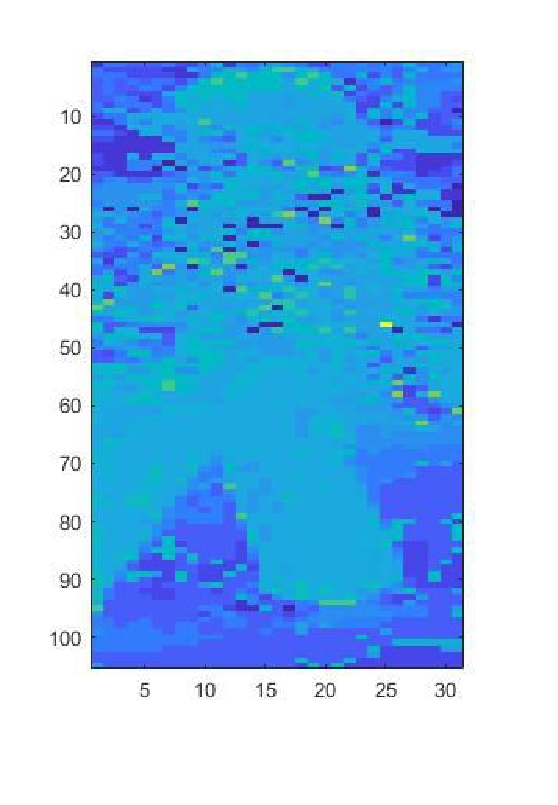
\includegraphics [width=0.25\textwidth] {ozadje.pdf}
	\end{center}
	\caption{S histogramom ozadja utežena regija tarče po kateri z Mean shift koraki iščemo maksimum. V primerjavi s sliko \ref{brezozadja} je tarča bolj razločna. Sekvenca 'woman'.}
	\label{ozadje}
\end{figure}

\begin{figure}[h]
	\begin{center}
		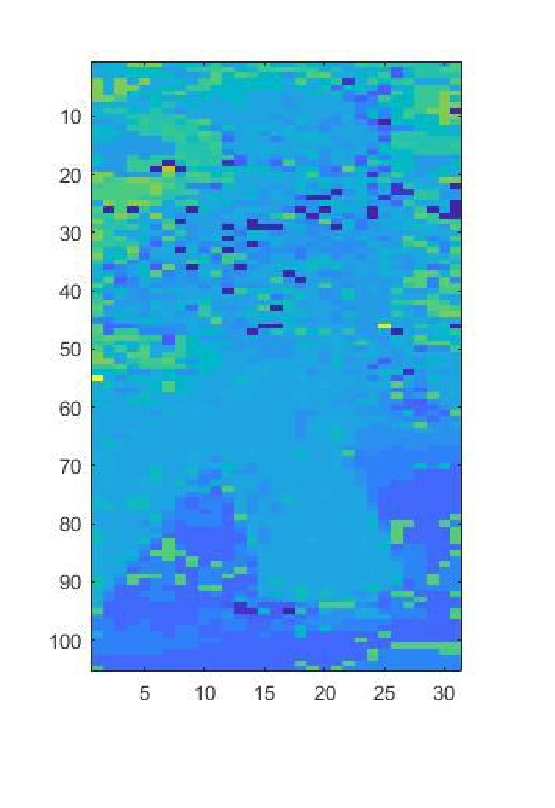
\includegraphics [width=0.25\textwidth] {brezozadja.pdf}
	\end{center}
	\caption{Neutežena regija tarče po kateri z Mean shift koraki iščemo maksimum. Sekvenca 'woman'.}
	\label{brezozadja}
\end{figure}

Tudi histogram ozadja B skozi sekvenco postopoma posodabljamo glede na podobnost regije s predlogo: 

$B = (1-beta)*Bstari + beta*Bnovi$, 

kjer je beta določen kot : $beta = alfa*10$.

\subsection{Parametra Kalmanovega filtra}
Kot smo omenili v poglvju 2.4 na delovanje vplivamo s parametroma $k_q$ in $k_r$. $k_q$ smo določili v inicializaciji glede na delež slike, ki ga pokriva tarča. To je potrebno, da je velikost kovariance razmeroma enaka v vseh sekvencah glede na velikost tarče:

$k_q = (wTarget*hTarget)/(wFrame*hFrame)*delta$. 

Pri modelih NCV in NCA ima delta vrednost 5, pri modelu RW pa 50, ker je velikost variance manjša pri RW. Pri RW namreč upoštevamo le položaj tarče. 

Vrednost $k_r$ določimo v vsaki sliki glede na podobnost histograma izbrane regije s predlogo $k_r = omega*(1-simil)$. Omega je faktor odvisen od velikost tarče: 

$omega = wTarget*hTarget)/(wFrame*hFrame)*2000$. 

Če se regija tarče razteza se mora povečati tudi kovarianca, saj lahko zgrešimo za več pikslov kot pa če je tarča majhna. Poleg tega nam to pomaga, ko se regija raztegne zaradi bližine tarči podobnega objekta. Takrat je koristno zmanjšati vpliv meritve in zaupati dinamičnemu modelu. Množenje z 2000 poveča vpliv raztezanja na kovarianco.

\section{Testiranje}
\subsection{Glajenje funkcije}
Najprej bomo testirali sam Kalmanov filter na primeru glajenja točk funkcije.
Spodaj so predstavljeni rezultati testiranja vpliva različnih modelov gibanja in vrednosti parametrov $k_q$, $k_r$ na Kalmanov filter. Za časovni korak $T$ smo predpostavili, da ima vedno vrednost 1.

V primeru spiralne krivulje s 40 točkami in vrednosti parametra $k_q = k_r = 1$ je vpliv šuma majhen tako na meritve kot na model gibanja. Na sliki \ref{q1r1} lahko vidimo vpliv modela gibanja na Kalmanov filter. Razvidno je da model NCV malo zaostaja za meritvami, saj ne upošteva dovolj pospeška (krivulja meritev se postopama zmanjšuje).
\begin{figure}[h]
	\begin{center}
		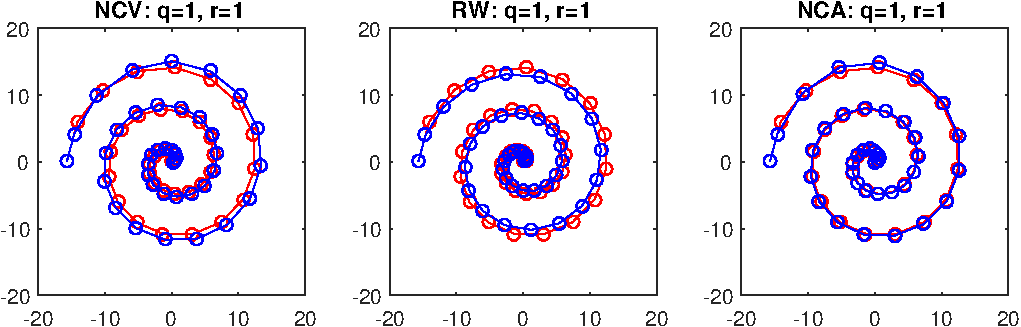
\includegraphics [width=0.45\textwidth] {q1r1.pdf}
	\end{center}
	\caption{Glajenje meritev (rdeča krivulja) s Kalmanovim filtrom (modra krivulja) pri modelih gibanja RW, NCV in NCA ter parametrom $k_q=1, r=1$. }
	\label{q1r1}
\end{figure}  

RW model upošteva le položaj in zato le približno sledi krivulji meritev. 
NCA na začetku sledi podobno kot NCV, kasneje pa se zaradi upoštevanja pospeška lepše prilagodi krivulji meritev. Enak graf dobimo za vse vrednosti pri katerih sta $k_q$ in $k_r$ enaka - Kalmanov filter za napovedovanje enakovredno upošteva meritve in model gibanja, saj je varianca (posledično šum) pri obeh ista (slika  \ref{q100r100}).
\begin{figure}[h]
	\begin{center}
		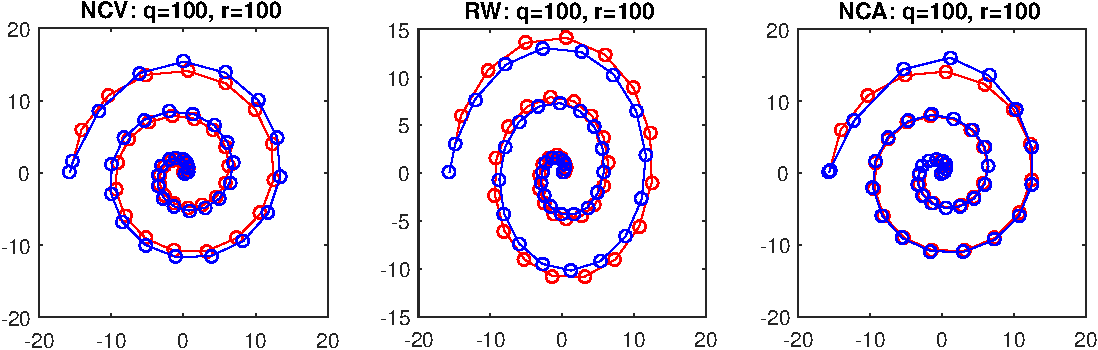
\includegraphics [width=0.45\textwidth] {q100r100.pdf}
	\end{center}
	\caption{Glajenje meritev (rdeča krivulja) s Kalmanovim filtrom (modra krivulja) pri modelih gibanja RW, NCV in NCA ter parametrom $k_q=100, k_r=100$. }
	\label{q100r100}
\end{figure}  

Če $k_r$ pustimo majnen, povečamo pa vrednost parametra $k_q$ in s tem šum modela gibanja opazimo (na sliki \ref{q5r1}), da se krivulje modelov obnošajo enako kot prej, le da se sedaj bolj prilegajo krivulji meritev. Če efekt pojačamo in vrednost $k_q$ močno povečamo, lahko na sliki \ref{q100r1} vidimo, da se Kalmanove krivulje popolnoma ujemajo z meritvami - vpliv modela je izničen. Takšno delovanje je posledica velikega šuma modela, zaradi katerega pri filtriranju upoštevamo le meritve - vrednosti modela se preveč razlikujejo od meritev, da bi jih še upoštevali.
\begin{figure}[h]
	\begin{center}
		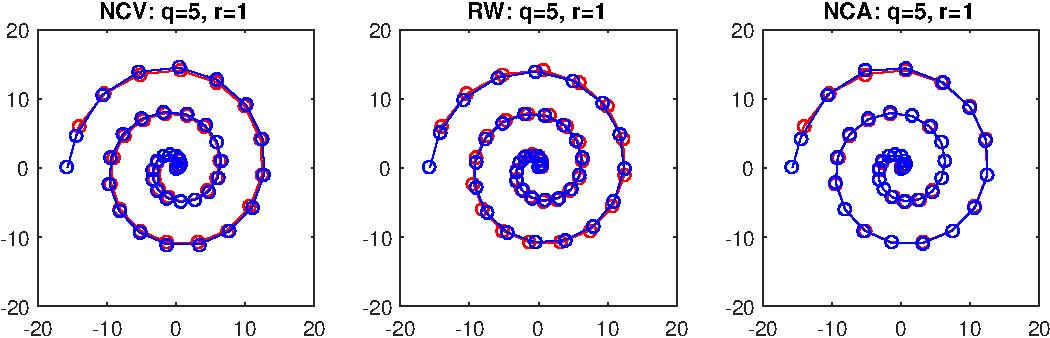
\includegraphics [width=0.45\textwidth] {q5r1.pdf}
	\end{center}
	\caption{Glajenje meritev (rdeča krivulja) s Kalmanovim filtrom (modra krivulja) pri modelih gibanja RW, NCV in NCA ter parametrom $k_q=5, k_r=1$. }
	\label{q5r1}
\end{figure} 
\begin{figure}[h]
	\begin{center}
		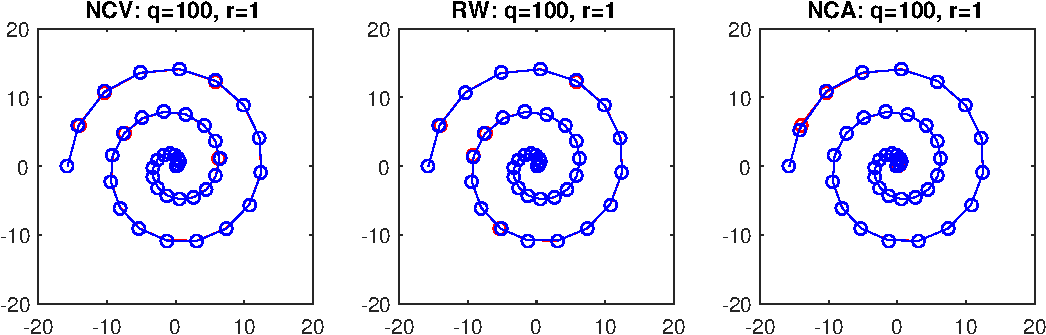
\includegraphics [width=0.45\textwidth] {q100r1.pdf}
	\end{center}
	\caption{Glajenje meritev (rdeča krivulja) s Kalmanovim filtrom (modra krivulja) pri modelih gibanja RW, NCV in NCA ter parametrom $k_q=100, k_r=1$. }
	\label{q100r1}
\end{figure}   

Obratno delovanje lahko opazimo na sliki \ref{q1r5} in \ref{q1r100}.  Vrednosti meritev so preveč šumne v primerjavi z napovedmi, zato se upošteva bolj model gibanja. NCA in NCV še vedno približno ohranita obliko spirale (NCV bolje kot NCA saj pospešek NCA pokvari obliko), medtem ko se model RW popolnoma izrodi, ker je večinsko odvisen le od položaja.
\begin{figure}[h]
	\begin{center}
		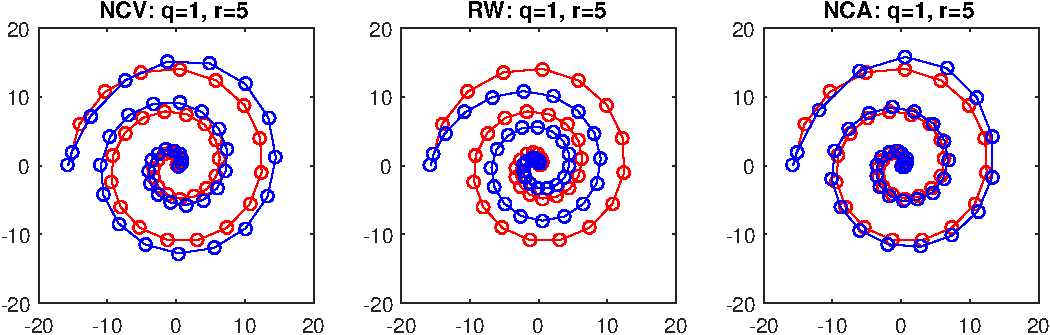
\includegraphics [width=0.45\textwidth] {q1r5.pdf}
	\end{center}
	\caption{Glajenje meritev (rdeča krivulja) s Kalmanovim filtrom (modra krivulja) pri modelih gibanja RW, NCV in NCA ter parametrom $k_q=1, k_r=5$. }
	\label{q1r5}
\end{figure}  
\begin{figure}[h]
	\begin{center}
		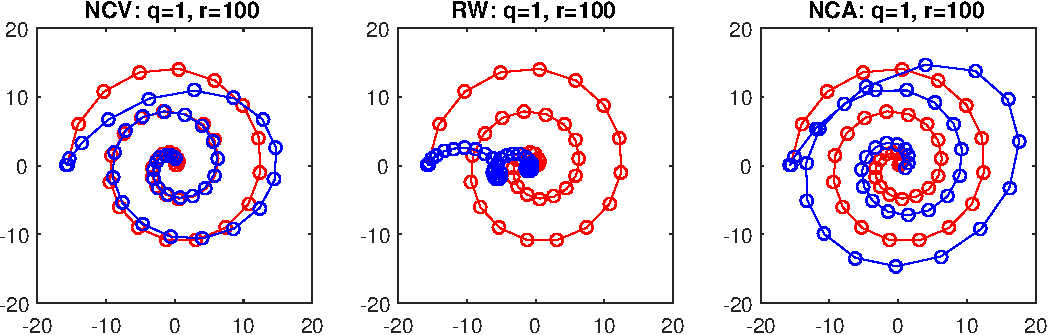
\includegraphics [width=0.45\textwidth] {q1r100.pdf}
	\end{center}
	\caption{Glajenje meritev (rdeča krivulja) s Kalmanovim filtrom (modra krivulja) pri modelih gibanja RW, NCV in NCA ter parametrom $k_q=1, k_r=100$. }
	\label{q1r100}
\end{figure}  

Pri sinusni krivulji s polovico številom točk (N = 20) je delovanje podobno, le da se Kalmanova krivulja bolje prilega meritvam, saj v primerjavi s spiralo, ne spreminja konstantno smeri (slika \ref{sinq1r1}). Na sliki \ref{sinq1r100} lahko vidimo upoštevanje samo dinamičnega modela. NCV zgladi meritve v bolj položno a manjšo krivuljo, RW preveč zgladi in se izroji, NCA pa se približno prilagodi meritvam. 
\begin{figure}[h]
	\begin{center}
		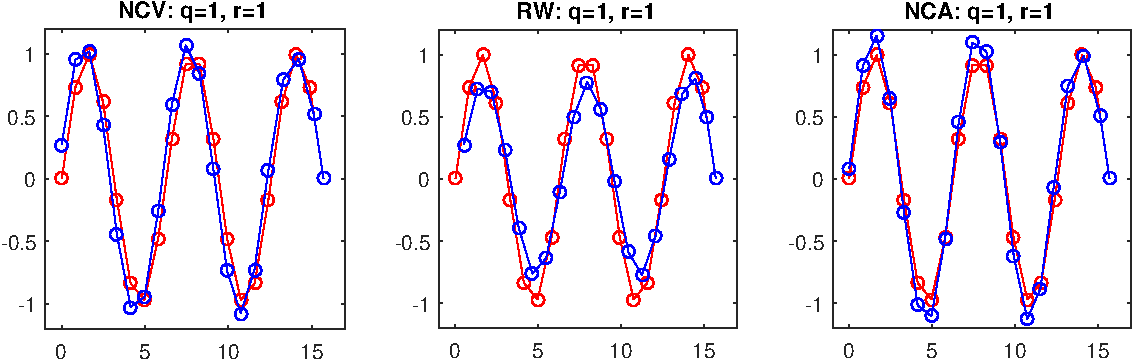
\includegraphics [width=0.45\textwidth] {sinq1r1.pdf}
	\end{center}
	\caption{Glajenje meritev (rdeča krivulja) s Kalmanovim filtrom (modra krivulja) pri modelih gibanja RW, NCV in NCA ter parametrom $k_q=1, k_r=1$. }
	\label{sinq1r1}
\end{figure} 
\begin{figure}[h]
	\begin{center}
		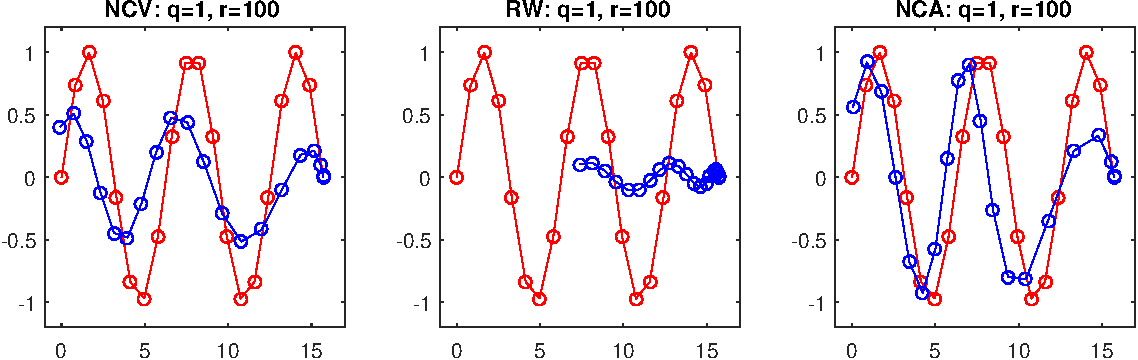
\includegraphics [width=0.45\textwidth] {sinq1r100.pdf}
	\end{center}
	\caption{Glajenje meritev (rdeča krivulja) s Kalmanovim filtrom (modra krivulja) pri modelih gibanja RW, NCV in NCA ter parametrom $k_q=1, k_r=100$. }
	\label{sinq1r100}
\end{figure} 

Pri testiranju na gaussovi krivulji, z 20 točkami, lahko lepo vidimo vpliv modelov gibanja (slika \ref{gaq1r1}). Model RW zgladi meritve krivulje in se ustavi pravočasno, ko ta pada na desni strani. NCV zaradi upoštevanja hitrosti nadaljuje glajenje čez spodnjo mejo krivulje preden se vrne v ravnovesno lego. Model NCA zaradi upoštevanja pospeška, nadaljuje glajenje čez spodnjo mejo ter nato preveč naraste preden doseže ravnovesno lego (naredi nekakšno nihanje).
\begin{figure}[h]
	\begin{center}
		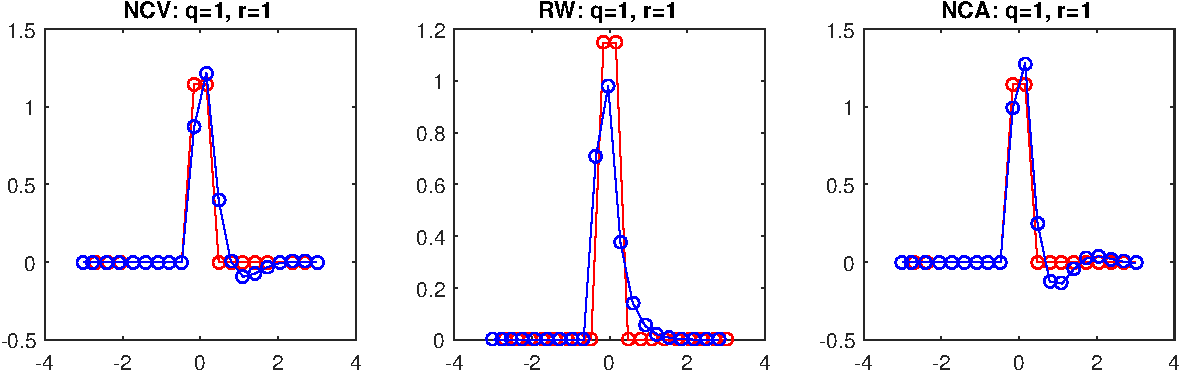
\includegraphics [width=0.45\textwidth] {gaq1r1.pdf}
	\end{center}
	\caption{Glajenje meritev (rdeča krivulja) s Kalmanovim filtrom (modra krivulja) pri modelih gibanja RW, NCV in NCA ter parametrom $k_q=1, k_r=1$. }
	\label{gaq1r1}
\end{figure} 

\subsection{Sledenje}
Kalmanov filter smo na primeru sledenja testirali z različnimi modeli gibanja. Testi so bili izvedeni na testni sekvencah slik vot2014 (http://box.vicos.si/vot/vot2014.zip) z uporabo ogrodja Tracking Evaluation Toolkit \\ (https://github.com/alanlukezic/tracking-toolkit-lite). Za ocenjevanje delovanja sta definirani meri prekritje (angl. overlap) - kolikšen delež tarče pokriva naš sledilnik skozi sekvenco in število odpovedi (angl. failures) - kolikokrat naš sledilnik odpove, ker izgubi tarčo in ga je potrebno reinicializirati. 

\subsubsection{Brez dinamičnega modela}
Najprej smo testirali delovanje Mean shift (MS) sledilnika brez Kalmanovega filtra, da lahko v nadaljevanju primerjamo delovanje in vidimo, kje običajni sledilnik deluje boljše in slabše. 

V tebeli \ref{tabelams} lahko razberemo delovanje slednilnika. V večini primerov se obnese dobro. Brez odpovedi prenese tudi sekvence kot je npr. 'sunshade', kjer je veliko hitrih gibov. Odpove pa v primerih, kjer pride do zakritja tarče (slika \ref{msjogging} ali ob kratkemu zaporedju napačnih zaznav (slika \ref{msmoto}) ter bližini tarči podobnega predmeta (slika \ref{mshand}).

\begin{table}[h!]
	\begin{center}
		\begin{tabular}{l c c}
			\hline 
			& \multicolumn{2}{c}{{\bf MS}}\\
			{\bf Sequence} & {\bf Overlap} & {\bf Failures} \\
			\hline 
			ball & 0.75 & 0\\
			basketball & 0.63 & 2\\
			bicycle & 0.40 & 0\\
			bolt & 0.50 & 2\\
			car & 0.57 & 0\\
			david & 0.29 & 1\\
			diving & 0.37 & 0\\
			drunk & 0.53 & 0\\
			fernando & 0.39 & 1\\
			fish1 & 0.18 & 3\\
			fish2 & 0.36 & 1\\
			gymnastics & 0.62 & 0\\
			hand1 & 0.48 & 0\\
			hand2 & 0.49 & 4\\
			jogging & 0.68 & 2\\
			motocross & 0.48 & 4\\
			polarbear & 0.58 & 0\\
			skating & 0.42 & 1\\
			sphere & 0.51 & 0\\
			sunshade & 0.56 & 0\\
			surfing & 0.52 & 0\\
			torus & 0.52 & 1\\
			trellis & 0.42 & 1\\
			tunnel & 0.43 & 6\\
			woman & 0.46 & 1\\
			\hline 
			{\bf Average} & 0.49 & 1.20\\
			\hline 
		\end{tabular}
	\end{center}
	\caption{Rezultati testiranja sledilnika brez modela gibanja na testnih sekvencah vot2014.}
	\label{tabelams}
\end{table}

\begin{figure}[h]
	\begin{center}
		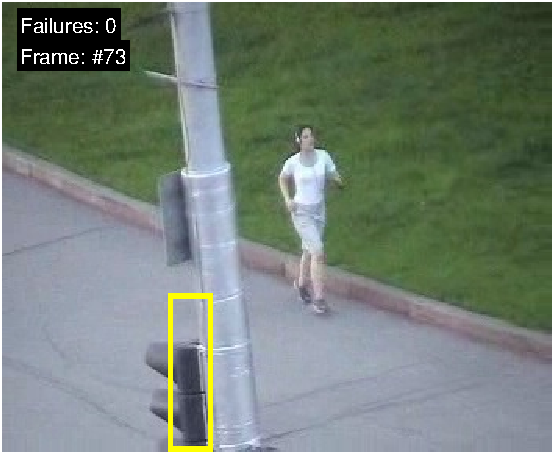
\includegraphics [width=0.45\textwidth] {msjogging.pdf}
	\end{center}
	\caption{Primer zakritja tarče za drogom in posledične odpovedi sledilnika brez dinamičnega modela. Sekvenca 'jogging'.}
	\label{msjogging}
\end{figure}
\begin{figure}[h]
	\begin{center}
		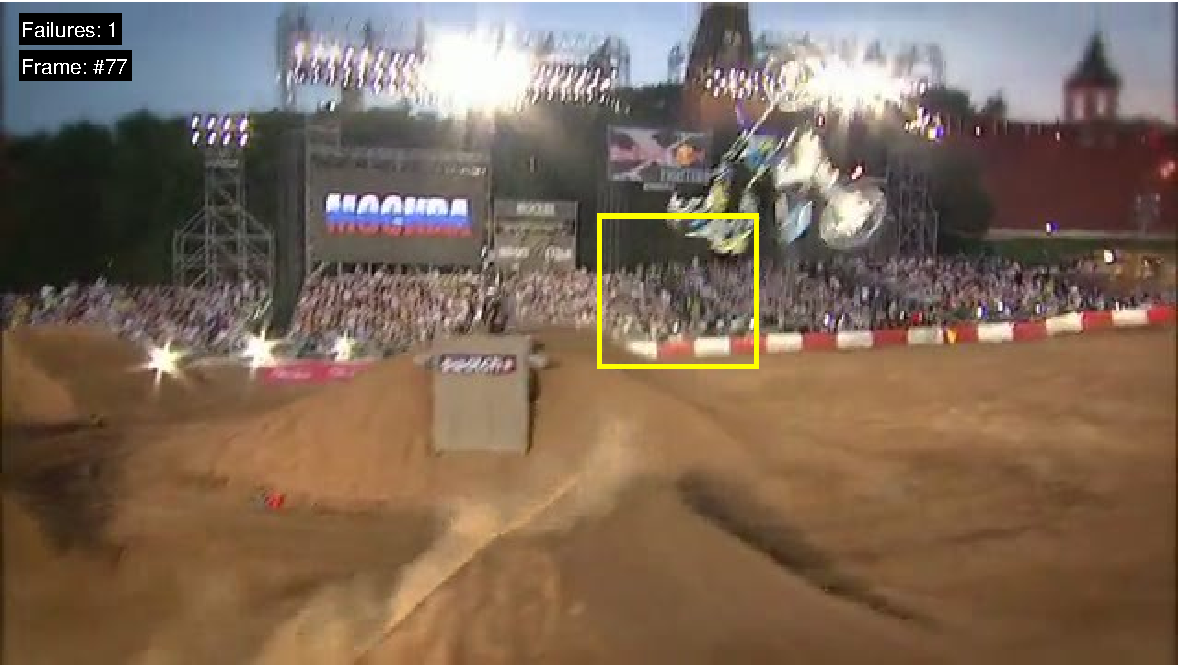
\includegraphics [width=0.45\textwidth] {msmoto.pdf}
	\end{center}
	\caption{Sledilnik brez dinamičnega modela je v prikazani sliki napačno zaznal tarčo, kar privede do odpovedi. Sekvenca 'motocross'.}
	\label{msmoto}
\end{figure}
\begin{figure}[h]
	\begin{center}
		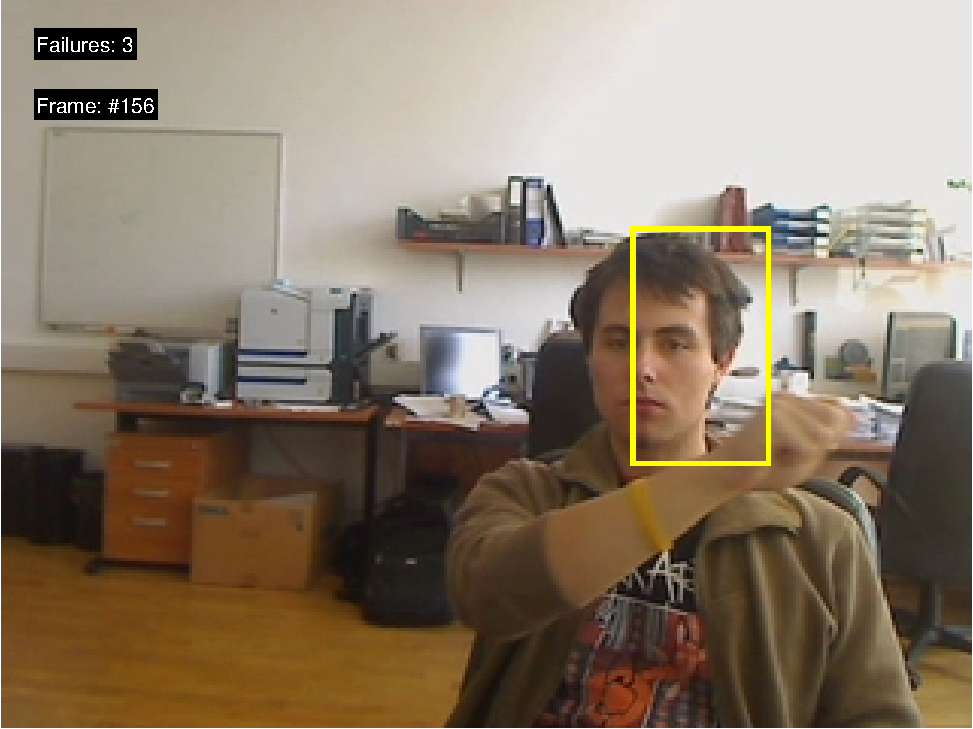
\includegraphics [width=0.45\textwidth] {mshand.pdf}
	\end{center}
	\caption{Sledilnik brez dinamičnega modela zaradi bližine tarči podobnega objekta odpove. Sekvenca 'hand2'.}
	\label{mshand}
\end{figure}

\subsubsection{RW model}
Kalmanov filter z modelom gibanja RW (random walk) deluje kot nekakšna zakasnitev. RW model namreč pri predvidevanju ne upošteva hitrosti ali pospeška ampak samo položaj. Tako za predikcijo izbere lokacijo prejšne slike (angl. frame) s kovarianco določeno s parametrom $k_q$. 

Važno je, da je kovarianca dinamičnega modela malo manjša od kovariance meritev, tako da ob pravilnih meritvah le malo upošteva predikcijo. Ko algoritem zazna negotovost meritve se kovarianca meritev poveča in upoštevamo predikcijo.  

V tebeli \ref{tabelarw} lahko razberemo delovanje slednilnika z RW modelom. Na splošno deluje slabše saj pri sekvencah s hitrimi premiki, zaradi predikcije preveč zaostaja in izgubi tarčo (slika \ref{rwball}. Zelo dobro pa se obnese v sekvenci 'jogging', ki vsebuje pokritje - dovolj dolgo ohranja prejšnje stanje, da se tarča pojavi spet pojavi, meritve postanejo zanesljive in lahko sledimo naprej (slike \ref{rwjogging1}, \ref{rwjogging2}, \ref{rwjogging3}). 

\begin{table}[h!]
	\begin{center}
		\begin{tabular}{l c c}
			\hline 
			& \multicolumn{2}{c}{{\bf MSRW}}\\
			{\bf Sequence} & {\bf Overlap} & {\bf Failures} \\
			\hline 
			ball & 0.69 & 1\\
			basketball & 0.61 & 2\\
			bicycle & 0.33 & 0\\
			bolt & 0.46 & 2\\
			car & 0.52 & 0\\
			david & 0.40 & 1\\
			diving & 0.38 & 0\\
			drunk & 0.53 & 0\\
			fernando & 0.36 & 1\\
			fish1 & 0.15 & 2\\
			fish2 & 0.33 & 1\\
			gymnastics & 0.62 & 0\\
			hand1 & 0.41 & 4\\
			hand2 & 0.46 & 7\\
			jogging & 0.59 & 0\\
			motocross & 0.31 & 1\\
			polarbear & 0.59 & 0\\
			skating & 0.43 & 1\\
			sphere & 0.43 & 0\\
			sunshade & 0.48 & 6\\
			surfing & 0.46 & 0\\
			torus & 0.41 & 1\\
			trellis & 0.41 & 1\\
			tunnel & 0.36 & 4\\
			woman & 0.43 & 1\\
			\hline 
			{\bf Average} & 0.45 & 1.44\\
			\hline 
		\end{tabular}
	\end{center}
	\caption{Rezultati testiranja sledilnika z RW modelom gibanja na testnih sekvencah vot2014.}
	\label{tabelarw}
\end{table}

\begin{figure}[h]
	\begin{center}
		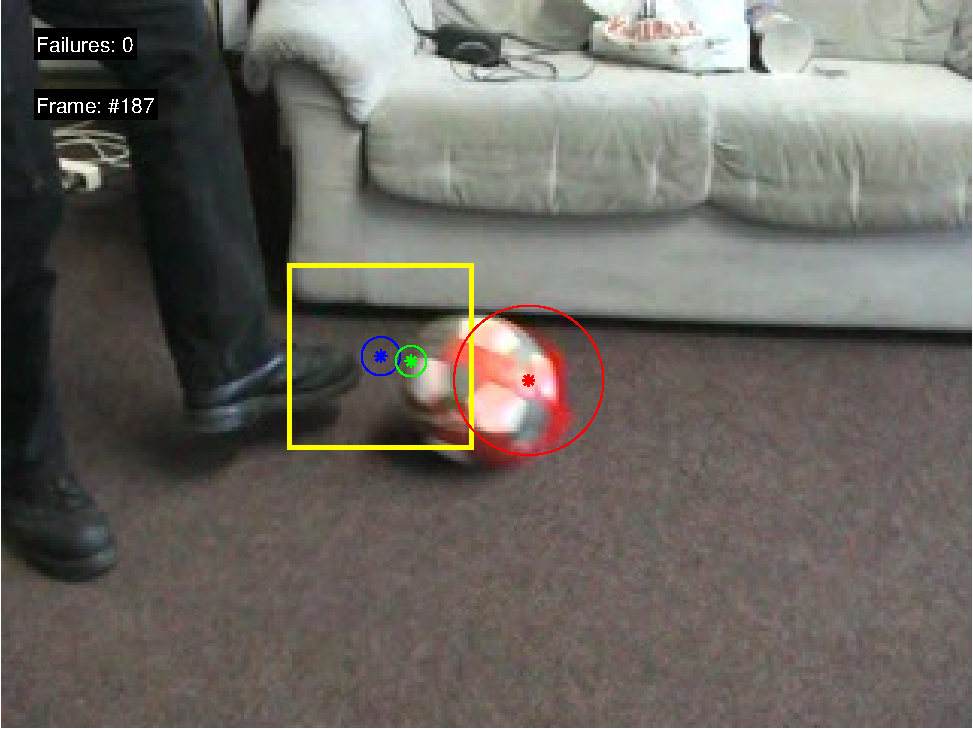
\includegraphics [width=0.45\textwidth] {rwball.pdf}
	\end{center}
	\caption{Sledilnik z modelom gibanja RW zaradi velikega premika neuspešno lokalizira tarčo. Modri krog prikazuje velikost variance (negotoviosti) predikcije, rdeči varianco meritve, zeleni pa končno stanje in njegovo varianco. Sekvenca 'ball'.}
	\label{rwball}
\end{figure}
\begin{figure}[h!]
	\begin{center}
		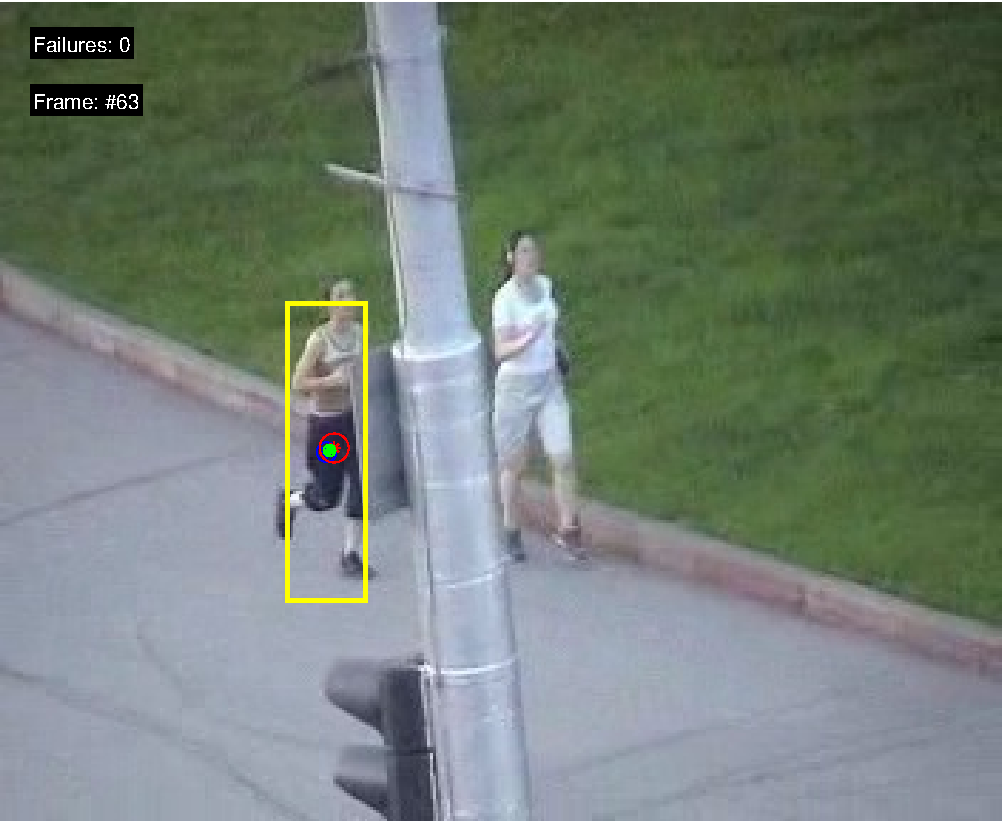
\includegraphics [width=0.45\textwidth] {rwjogging1.pdf}
	\end{center}
	\caption{Delovanje sledilnika z modelom gibanja RW na sekvenci 'jogging'. Modri krog prikazuje velikost variance (negotovost) predikcije, rdeči varianco meritve, zeleni pa končno stanje in njegovo varianco. Ker je regija dobro opisuje tarčo je negotovost vseh členov majhna.}
	\label{rwjogging1}
\end{figure}
\begin{figure}[h!]
	\begin{center}
		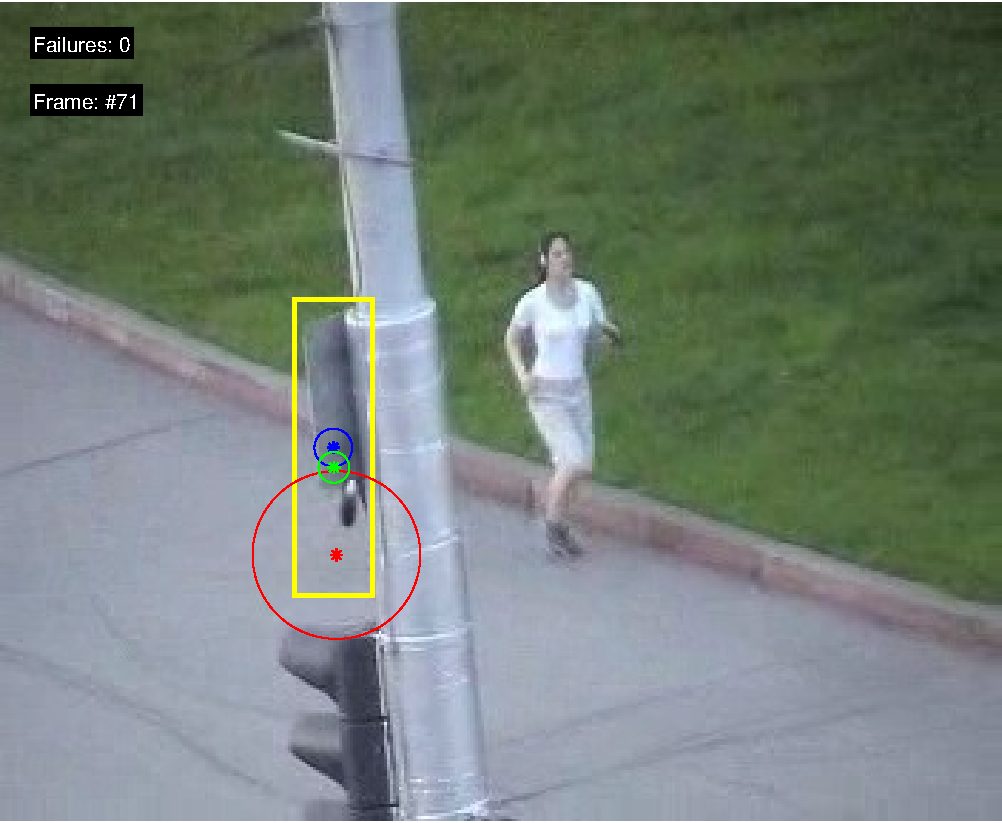
\includegraphics [width=0.45\textwidth] {rwjogging2.pdf}
	\end{center}
	\caption{Nadaljevanje slike \ref{rwjogging1}: delovanje sledilnika z modelom gibanja RW na sekvenci 'jogging'. Modri krog prikazuje velikost variance (negotovost) predikcije, rdeči varianco meritve, zeleni pa končno stanje in njegovo varianco. Tarča je prekrita zato z večjo gotovostjo upoštevamo predikcijo.}
	\label{rwjogging2}
\end{figure}
\begin{figure}[h!]
	\begin{center}
		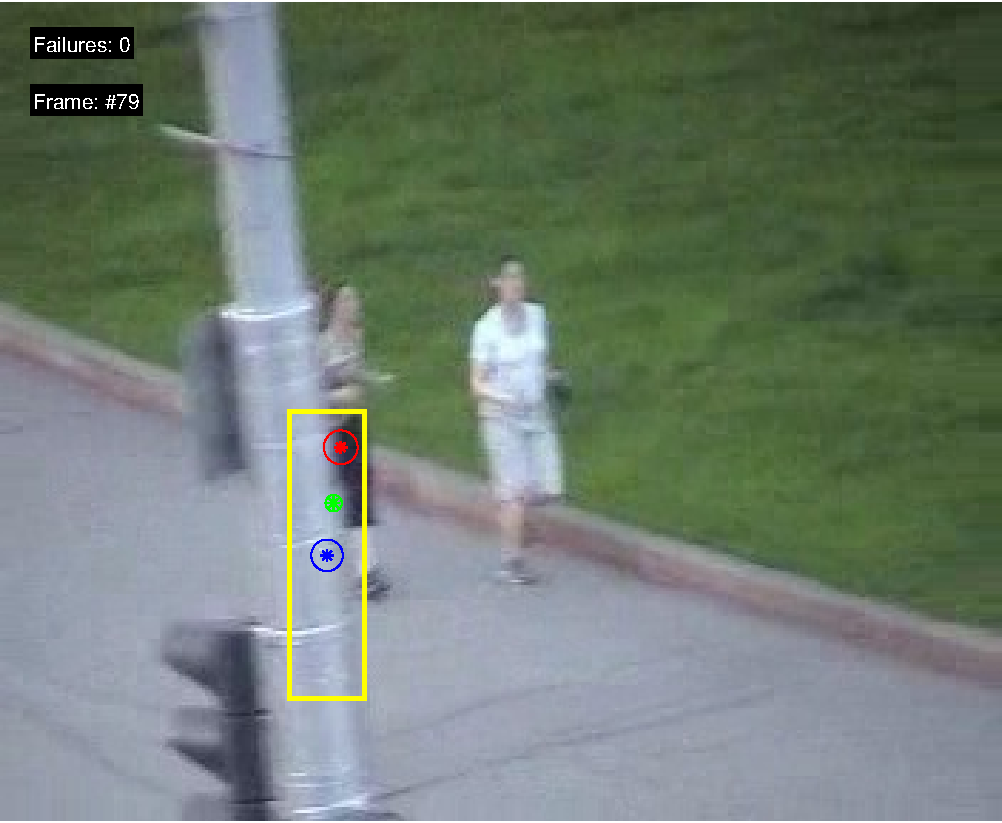
\includegraphics [width=0.45\textwidth] {rwjogging3.pdf}
	\end{center}
	\caption{Nadaljevanje slike \ref{rwjogging2}: delovanje sledilnika z modelom gibanja RW na sekvenci 'jogging'. Modri krog prikazuje velikost variance (negotovost) predikcije, rdeči varianco meritve, zeleni pa končno stanje in njegovo varianco. Tarča je prišla preko ovire zato nadaljujemo z večjim upoštevanjem meritve.}
	\label{rwjogging3}
\end{figure}

\subsubsection{NCV model}
Za razliko od RW modela, NCV pri predikciji upošteva še hitrost ter pospešek in ima zato večjo kovarianco predikcije. Zmožen je za nekaj sličic tudi nadaljevati pot tarče. To je koristno pri sekvencah, kot je 'motocross', kjer osnovni MS sledilnik izgubi tarčo zaradi nenadnega napačnega zaznavanja, z NCV modelom pa zaradi predikcije uspe slediti premikanju tarče (slika \ref{ncvmoto}). 
\begin{figure}[h]
	\begin{center}
		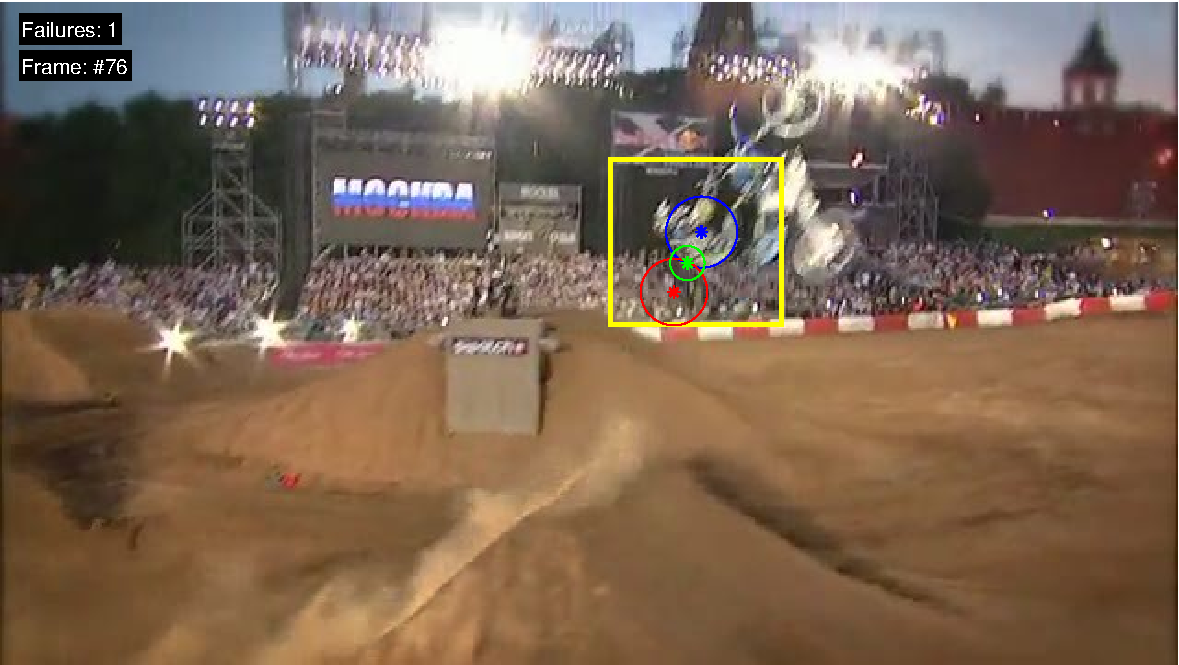
\includegraphics [width=0.45\textwidth] {ncvmoto.pdf}
	\end{center}
	\caption{Sledilnik z modelom gibanja NCV zaradi upoštevanja predikcije uspešno lokalizira tarčo, ki nadaljuje svoj pot. Modri krog prikazuje velikost variance (negotoviosti) predikcije, rdeči varianco meritve, zeleni pa končno stanje in njegovo varianco. Sekvenca 'motocross'.}
	\label{ncvmoto}
\end{figure}

V tebeli \ref{tabelarncv} lahko razberemo delovanje slednilnika z NCV modelom. Delovanje je malo boljše od RW modela, ker ne ohranja le prejšnega položaja. Zaradi tega pa tudi ni zmožen prenesti popolnega prekritja tarče pri sekvenci 'jogging'. Malo slabši je tudi od osnovnega MS sledilnika, ker zaradi večje velikosti kovariance ni zmožen dovolj popraviti slabe lastnosti sledilnika, hkrati pa upošteva malo varianco dovolj da pokvari hitre nenadne premike. 

\begin{table}[h!]
	\begin{center}
		\begin{tabular}{l c c}
			\hline 
			& \multicolumn{2}{c}{{\bf MSNCV}}\\
			{\bf Sequence} & {\bf Overlap} & {\bf Failures} \\
			\hline 
			ball & 0.73 & 0\\
			basketball & 0.63 & 2\\
			bicycle & 0.44 & 1\\
			bolt & 0.44 & 2\\
			car & 0.58 & 0\\
			david & 0.42 & 1\\
			diving & 0.37 & 0\\
			drunk & 0.53 & 0\\
			fernando & 0.37 & 1\\
			fish1 & 0.27 & 3\\
			fish2 & 0.36 & 1\\
			gymnastics & 0.59 & 1\\
			hand1 & 0.49 & 0\\
			hand2 & 0.31 & 4\\
			jogging & 0.48 & 1\\
			motocross & 0.40 & 3\\
			polarbear & 0.56 & 0\\
			skating & 0.40 & 1\\
			sphere & 0.44 & 0\\
			sunshade & 0.46 & 3\\
			surfing & 0.56 & 0\\
			torus & 0.50 & 1\\
			trellis & 0.35 & 1\\
			tunnel & 0.34 & 6\\
			woman & 0.45 & 1\\
			\hline 
			{\bf Average} & 0.46 & 1.32\\
			\hline 
		\end{tabular}
	\end{center}
	\caption{Rezultati testiranja sledilnika z NCV modelom gibanja na testnih sekvencah vot2014.}
	\label{tabelarncv}
\end{table}


\subsubsection{NCA model}
Sledilnik z NCA modelom upošteva hitrost, pospešek in sunke ter ima tako največjo varianco predikcije. V večini primerov upošteva meritve in le malo popravlja lokalizacijo. Zaradi tega lažje sledi hitrim premikom v primerjavi z  NCV in RW ter ni zmožen tako dobro popraviti pokritosti.

Kljub temu lahko v tabeli \ref{tabelanca} vidimo, da ima najmanj odpovedi. To je predvsem zato, ker se obnaša zelo podobno kot osnovni MS sledilnik, v nekaterih primerih pa ga le malo popravi, ko je kovarianca meritve velika (slika \ref{ncahand}). 

\begin{table}[h!]
	\begin{center}
		\begin{tabular}{l c c}
			\hline 
			& \multicolumn{2}{c}{{\bf MSNCA}}\\
			{\bf Sequence} & {\bf Overlap} & {\bf Failures} \\
			\hline 
			ball & 0.75 & 0\\
			basketball & 0.63 & 2\\
			bicycle & 0.38 & 0\\
			bolt & 0.39 & 2\\
			car & 0.57 & 0\\
			david & 0.31 & 1\\
			diving & 0.38 & 0\\
			drunk & 0.53 & 0\\
			fernando & 0.36 & 1\\
			fish1 & 0.06 & 0\\
			fish2 & 0.37 & 2\\
			gymnastics & 0.61 & 0\\
			hand1 & 0.45 & 0\\
			hand2 & 0.44 & 2\\
			jogging & 0.51 & 1\\
			motocross & 0.48 & 4\\
			polarbear & 0.57 & 0\\
			skating & 0.42 & 3\\
			sphere & 0.48 & 0\\
			sunshade & 0.55 & 0\\
			surfing & 0.58 & 0\\
			torus & 0.53 & 1\\
			trellis & 0.40 & 2\\
			tunnel & 0.39 & 5\\
			woman & 0.42 & 2\\
			\hline 
			{\bf Average} & 0.46 & 1.12\\
			\hline 
		\end{tabular}
	\end{center}
	\caption{Rezultati testiranja sledilnika z NCV modelom gibanja na testnih sekvencah vot2014.}
	\label{tabelanca}
\end{table}

\begin{figure}[h]
	\begin{center}
		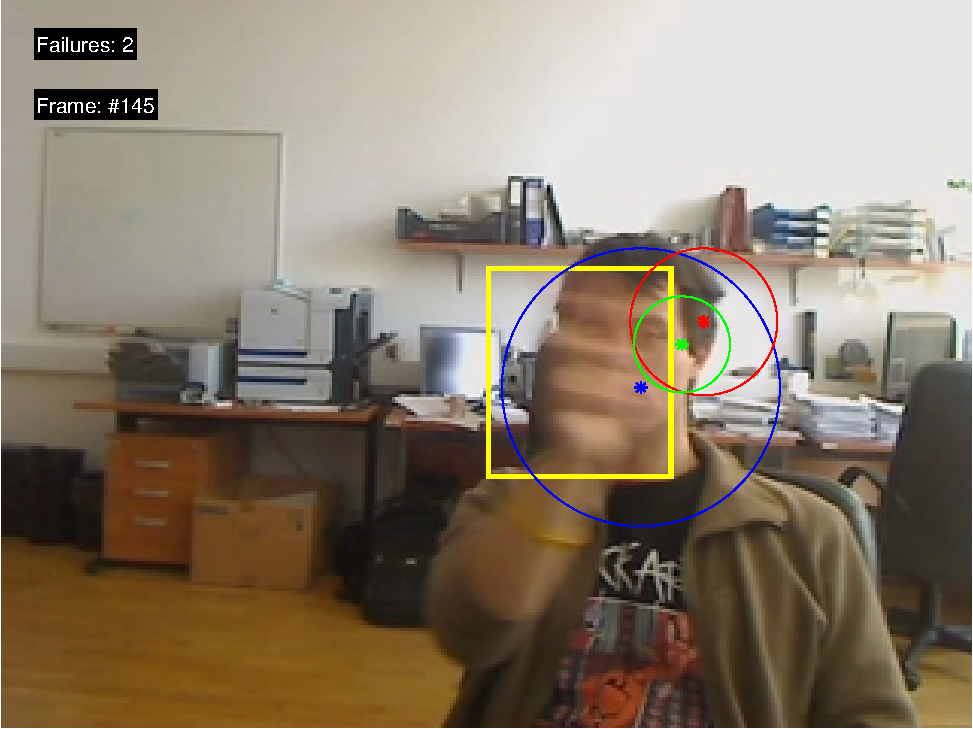
\includegraphics [width=0.45\textwidth] {ncahand.pdf}
	\end{center}
	\caption{Kljub veliki kovarianci predikcije sledilnika z modelom gibanja NCA, uspemo premakniti končno stanje dovolj, da se izognemo napačni meritvi. Modri krog prikazuje velikost variance (negotoviosti) predikcije, rdeči varianco meritve, zeleni pa končno stanje in njegovo varianco. Sekvenca 'hand2'.}
	\label{ncahand}
\end{figure}


\section{Zaključek}
Izpeljali in implementirali smo Kalmanov filter ter na praktičnem primeru preizkusili njegovo delovanje in s tem potrdili naše razumevanje teorije. 
%Parametra $k_q$ in $k_r$ je potrebno določiti glede na posamezni primer, vendar v večini primerov želimo, da se kovarianci predikcije in meritve ne razlikujeta preveč. Tako lahko dobro določimo novo stanje.

Dobro implementiran Mean shift sledilnik, z upoštevanjem ozadja in prilagajanjem skale se že sam obnese razmeroma dobro v večini sekvenc. Z dodajanjem Kalmanovega filtra smo poskusili izboljšati še tiste primere v katerih odpove - predvsem zakritost tarče in nenadne slabe detekcije. 

Pri testiranju modelov RW, NCV in NCA smo ugotovili, da če dovolj upoštevamo dinamični model, lahko  popravimo odpovedi v željenih primerih ampak pri tem lahko pokvarimo tudi že prej delujoče primere. Še posebno tiste pri katerih se tarča hitro premika. 

Zato se je najbolje obnesel NCA model, ki kljub temu, da ne popravi (popolnoma) težkih primerov, s svojo predikcijo malo izboljša osnovni algoritem. Primerjavo vseh modelov lahko vidimo na sliki \ref{ar} in tabeli \ref{tabela}. 

\begin{table*}[h]
	\begin{center}
		\begin{tabular}{l c c c c c c c c}
			\hline 
			& \multicolumn{2}{c}{{\bf MS}}& \multicolumn{2}{c}{{\bf MSRW}}& \multicolumn{2}{c}{{\bf MSNCV}}& \multicolumn{2}{c}{{\bf MSNCA}}\\
			{\bf Sequence} & {\bf Overlap} & {\bf Failures} & {\bf Overlap} & {\bf Failures} & {\bf Overlap} & {\bf Failures} & {\bf Overlap} & {\bf Failures} \\
			\hline 
			ball & 0.75 & 0 & 0.69 & 1 & 0.73 & 0 & 0.75 & 0\\
			basketball & 0.63 & 2 & 0.61 & 2 & 0.63 & 2 & 0.63 & 2\\
			bicycle & 0.40 & 0 & 0.33 & 0 & 0.44 & 1 & 0.38 & 0\\
			bolt & 0.50 & 2 & 0.46 & 2 & 0.44 & 2 & 0.39 & 2\\
			car & 0.57 & 0 & 0.52 & 0 & 0.58 & 0 & 0.57 & 0\\
			david & 0.29 & 1 & 0.40 & 1 & 0.42 & 1 & 0.31 & 1\\
			diving & 0.37 & 0 & 0.38 & 0 & 0.37 & 0 & 0.38 & 0\\
			drunk & 0.53 & 0 & 0.53 & 0 & 0.53 & 0 & 0.53 & 0\\
			fernando & 0.39 & 1 & 0.36 & 1 & 0.37 & 1 & 0.36 & 1\\
			fish1 & 0.18 & 3 & 0.15 & 2 & 0.27 & 3 & 0.06 & 0\\
			fish2 & 0.36 & 1 & 0.33 & 1 & 0.36 & 1 & 0.37 & 2\\
			gymnastics & 0.62 & 0 & 0.62 & 0 & 0.59 & 1 & 0.61 & 0\\
			hand1 & 0.48 & 0 & 0.41 & 4 & 0.49 & 0 & 0.45 & 0\\
			hand2 & 0.49 & 4 & 0.46 & 7 & 0.31 & 4 & 0.44 & 2\\
			jogging & 0.68 & 2 & 0.59 & 0 & 0.48 & 1 & 0.51 & 1\\
			motocross & 0.48 & 4 & 0.31 & 1 & 0.40 & 3 & 0.48 & 4\\
			polarbear & 0.58 & 0 & 0.59 & 0 & 0.56 & 0 & 0.57 & 0\\
			skating & 0.42 & 1 & 0.43 & 1 & 0.40 & 1 & 0.42 & 3\\
			sphere & 0.51 & 0 & 0.43 & 0 & 0.44 & 0 & 0.48 & 0\\
			sunshade & 0.56 & 0 & 0.48 & 6 & 0.46 & 3 & 0.55 & 0\\
			surfing & 0.52 & 0 & 0.46 & 0 & 0.56 & 0 & 0.58 & 0\\
			torus & 0.52 & 1 & 0.41 & 1 & 0.50 & 1 & 0.53 & 1\\
			trellis & 0.42 & 1 & 0.41 & 1 & 0.35 & 1 & 0.40 & 2\\
			tunnel & 0.43 & 6 & 0.36 & 4 & 0.34 & 6 & 0.39 & 5\\
			woman & 0.46 & 1 & 0.43 & 1 & 0.45 & 1 & 0.42 & 2\\
			\hline 
			{\bf Average} & 0.49 & 1.20 & 0.45 & 1.44 & 0.46 & 1.32 & 0.46 & 1.12\\
			\hline 
			\end{tabular}
	\end{center}
	\caption{Rezultati testiranja sledilnikov z različnimi modeli gibanja (brez modela gibanja, RW, NCV, NCA) na testnih sekvencah vot2014.}
	\label{tabela}
\end{table*}
\begin{figure*}[h]
	\begin{center}
		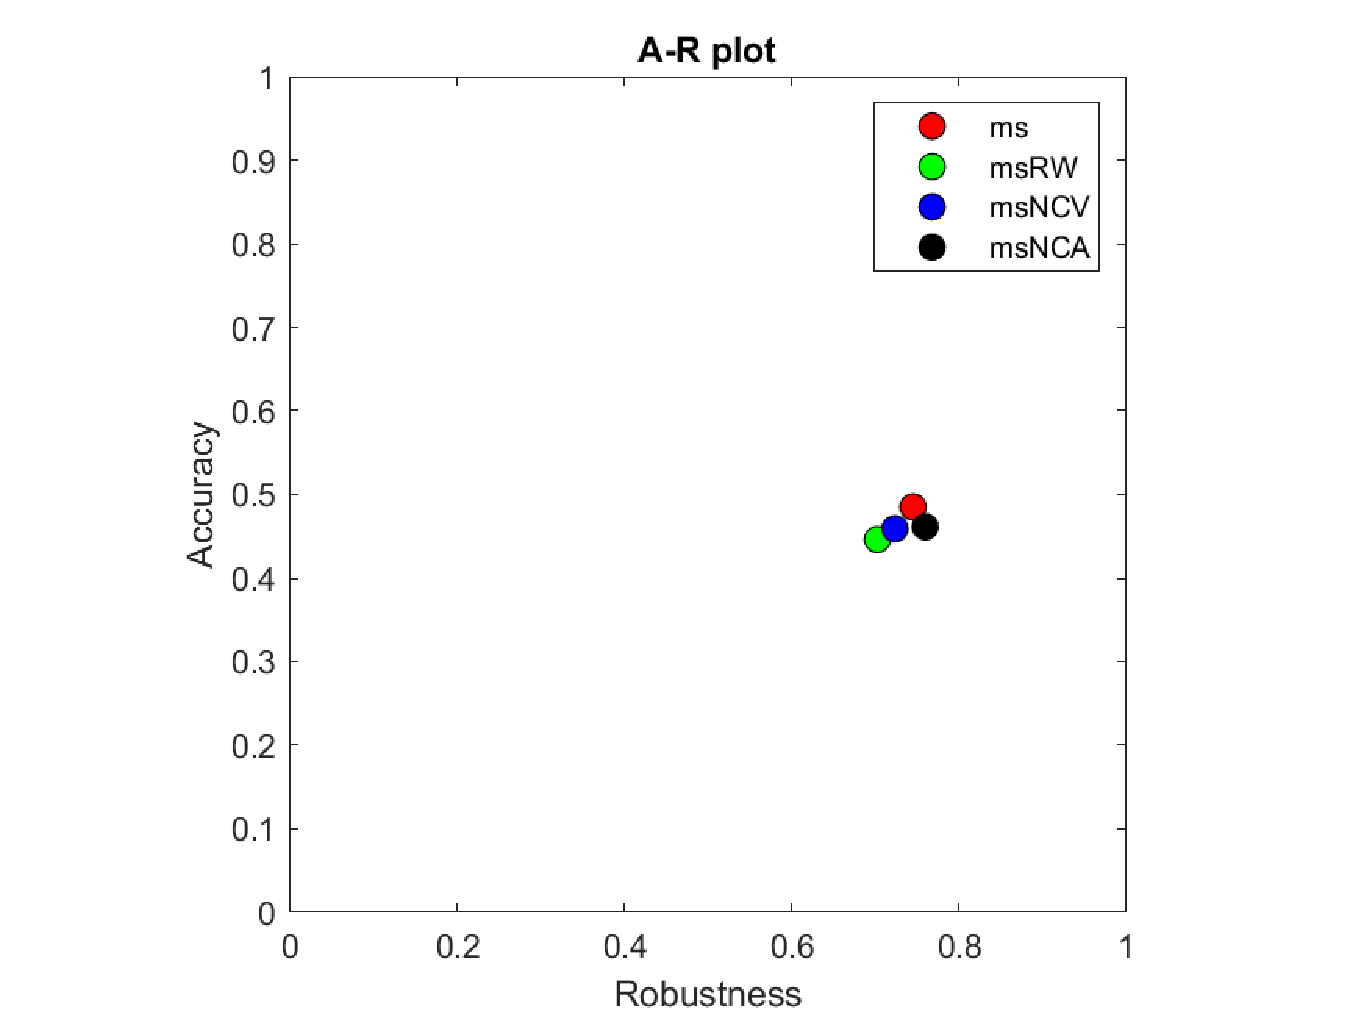
\includegraphics [width=1\textwidth] {ar.pdf}
	\end{center}
	\caption{A-R graf primerjave sledilnikov z različnimi modeli gibanja. }
	\label{ar}
\end{figure*} 


\small
\begin{thebibliography}{1}

\bibitem{prince} 
S. Prince,
\textit{Computer vision: models, learning and inference}. 
Cambridge University Press, 2012. (http://web4.cs.ucl.ac.uk/staff/s.prince/book/book.pdf)

\bibitem{clanek}
D. ,Comaniciu, V. Ramesh,P. Meer  
\textit{Kernel-based object tracking}.
IEEE Transactions on Pattern Analysis and Machine Intelligence, 2003

\end{thebibliography}

\end{document}
